%  article.tex (Version 3.3, released 19 January 2008)
%  Article to demonstrate format for SPIE Proceedings
%  Special instructions are included in this file after the
%  symbol %>>>>
%  Numerous commands are commented out, but included to show how
%  to effect various options, e.g., to print page numbers, etc.
%  This LaTeX source file is composed for LaTeX2e.

%  The following commands have been added in the SPIE class 
%  file (spie.cls) and will not be understood in other classes:
%  \supit{}, \authorinfo{}, \skiplinehalf, \keywords{}
%  The bibliography style file is called spiebib.bst, 
%  which replaces the standard style unstr.bst.  

\documentclass[]{spie}  %>>> use for US letter paper
%%\documentclass[a4paper]{spie}  %>>> use this instead for A4 paper
%%\documentclass[nocompress]{spie}  %>>> to avoid compression of citations
%% \addtolength{\voffset}{9mm}   %>>> moves text field down
%% \renewcommand{\baselinestretch}{1.65}   %>>> 1.65 for double spacing, 1.25 for 1.5 spacing 
%  The following command loads a graphics package to include images 
%  in the document. It may be necessary to specify a DVI driver option,
%  e.g., [dvips], but that may be inappropriate for some LaTeX 
%  installations. 
\usepackage[]{graphicx}
\usepackage{url}
\usepackage[table, xcdraw]{xcolor}
\usepackage{subcaption}

\title{3D scanning by means of dual-projector structured light illumination} 

%>>>> The author is responsible for formatting the 
%  author list and their institutions.  Use  \skiplinehalf 
%  to separate author list from addresses and between each address.
%  The correspondence between each author and his/her address
%  can be indicated with a superscript in italics, 
%  which is easily obtained with \supit{}.

\author{Daniel L. Lau\supit{a} and Ying Yu\supit{b}
\skiplinehalf
\supit{a}University of Kentucky, Address, Lexington, US; \\
\supit{b}University of Kentucky, Address, Lexington, US
}

%>>>> Further information about the authors, other than their 
%  institution and addresses, should be included as a footnote, 
%  which is facilitated by the \authorinfo{} command.

\authorinfo{Further author information: (Send correspondence to A.A.A.)\\A.A.A.: E-mail: aaa@tbk2.edu, Telephone: 1 505 123 1234\\  B.B.A.: E-mail: bba@cmp.com, Telephone: +33 (0)1 98 76 54 32}
%%>>>> when using amstex, you need to use @@ instead of @
 

%%%%%%%%%%%%%%%%%%%%%%%%%%%%%%%%%%%%%%%%%%%%%%%%%%%%%%%%%%%%% 
%>>>> uncomment following for page numbers
% \pagestyle{plain}    
%>>>> uncomment following to start page numbering at 301 
%\setcounter{page}{301} 
 
  \begin{document} 
  \maketitle 

%%%%%%%%%%%%%%%%%%%%%%%%%%%%%%%%%%%%%%%%%%%%%%%%%%%%%%%%%%%%% 
\begin{abstract}
This document shows the desired format and appearance of a manuscript prepared for the Proceedings of the SPIE.  It contains general formatting instructions and hints about how to use LaTeX.  The LaTeX source file that produced this document, {\tt article.tex} (Version 3.3), provides a template, used in conjunction with {\tt spie.cls} (Version 3.3).  
\end{abstract}

%>>>> Include a list of keywords after the abstract 

\keywords{Manuscript format, template, SPIE Proceedings, LaTeX}

%%%%%%%%%%%%%%%%%%%%%%%%%%%%%%%%%%%%%%%%%%%%%%%%%%%%%%%%%%%%%
\section{INTRODUCTION}
\label{sec:intro}  % \label{} allows reference to this section
Structured light illumination 

\section{HDMI}
HDMI is the abbreviation of High-Definition Multimedia Interface, it is one of the most popular diaplay interfaces. The newest release, HDMI Version 2.1 supports up to $10K$ video at $120 Hz$.
%\begin{figure}
%   \begin{center}
%   \begin{tabular}{c}
%   %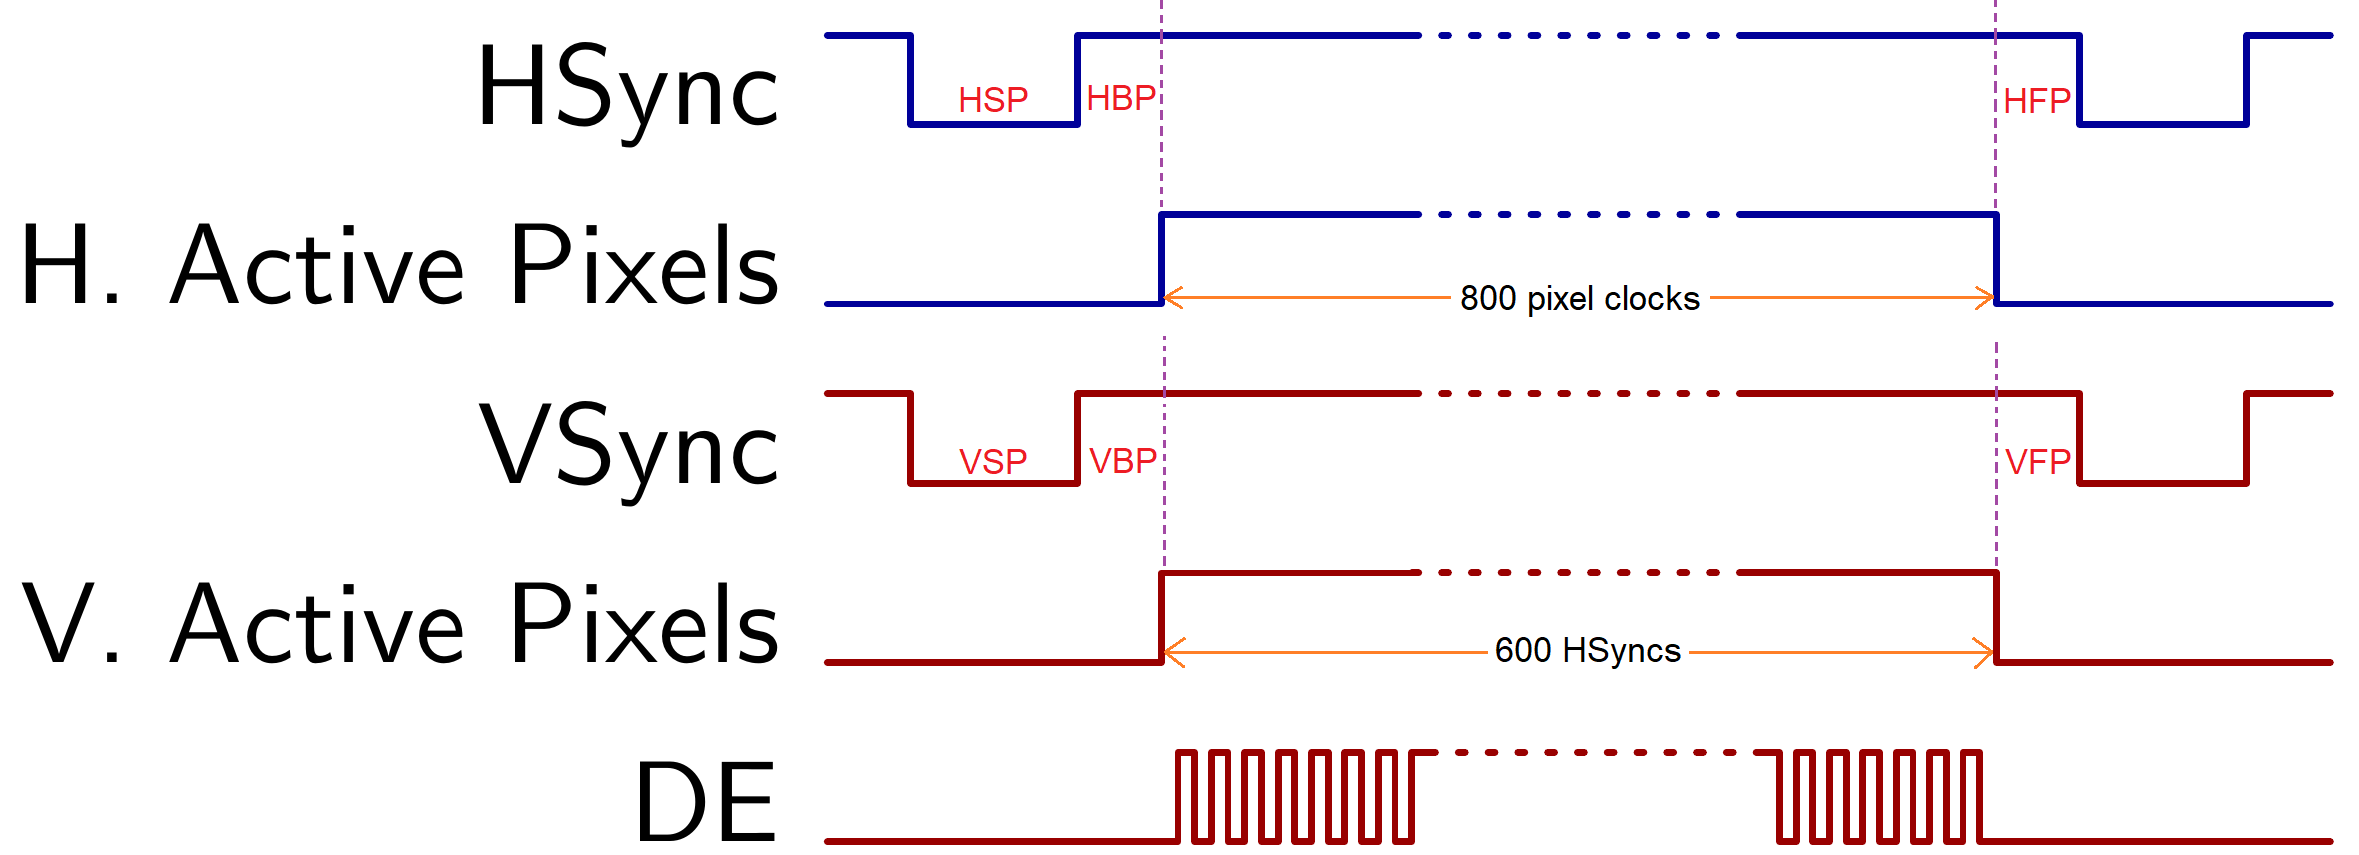
\includegraphics[height=7cm]{wf3.png}
%   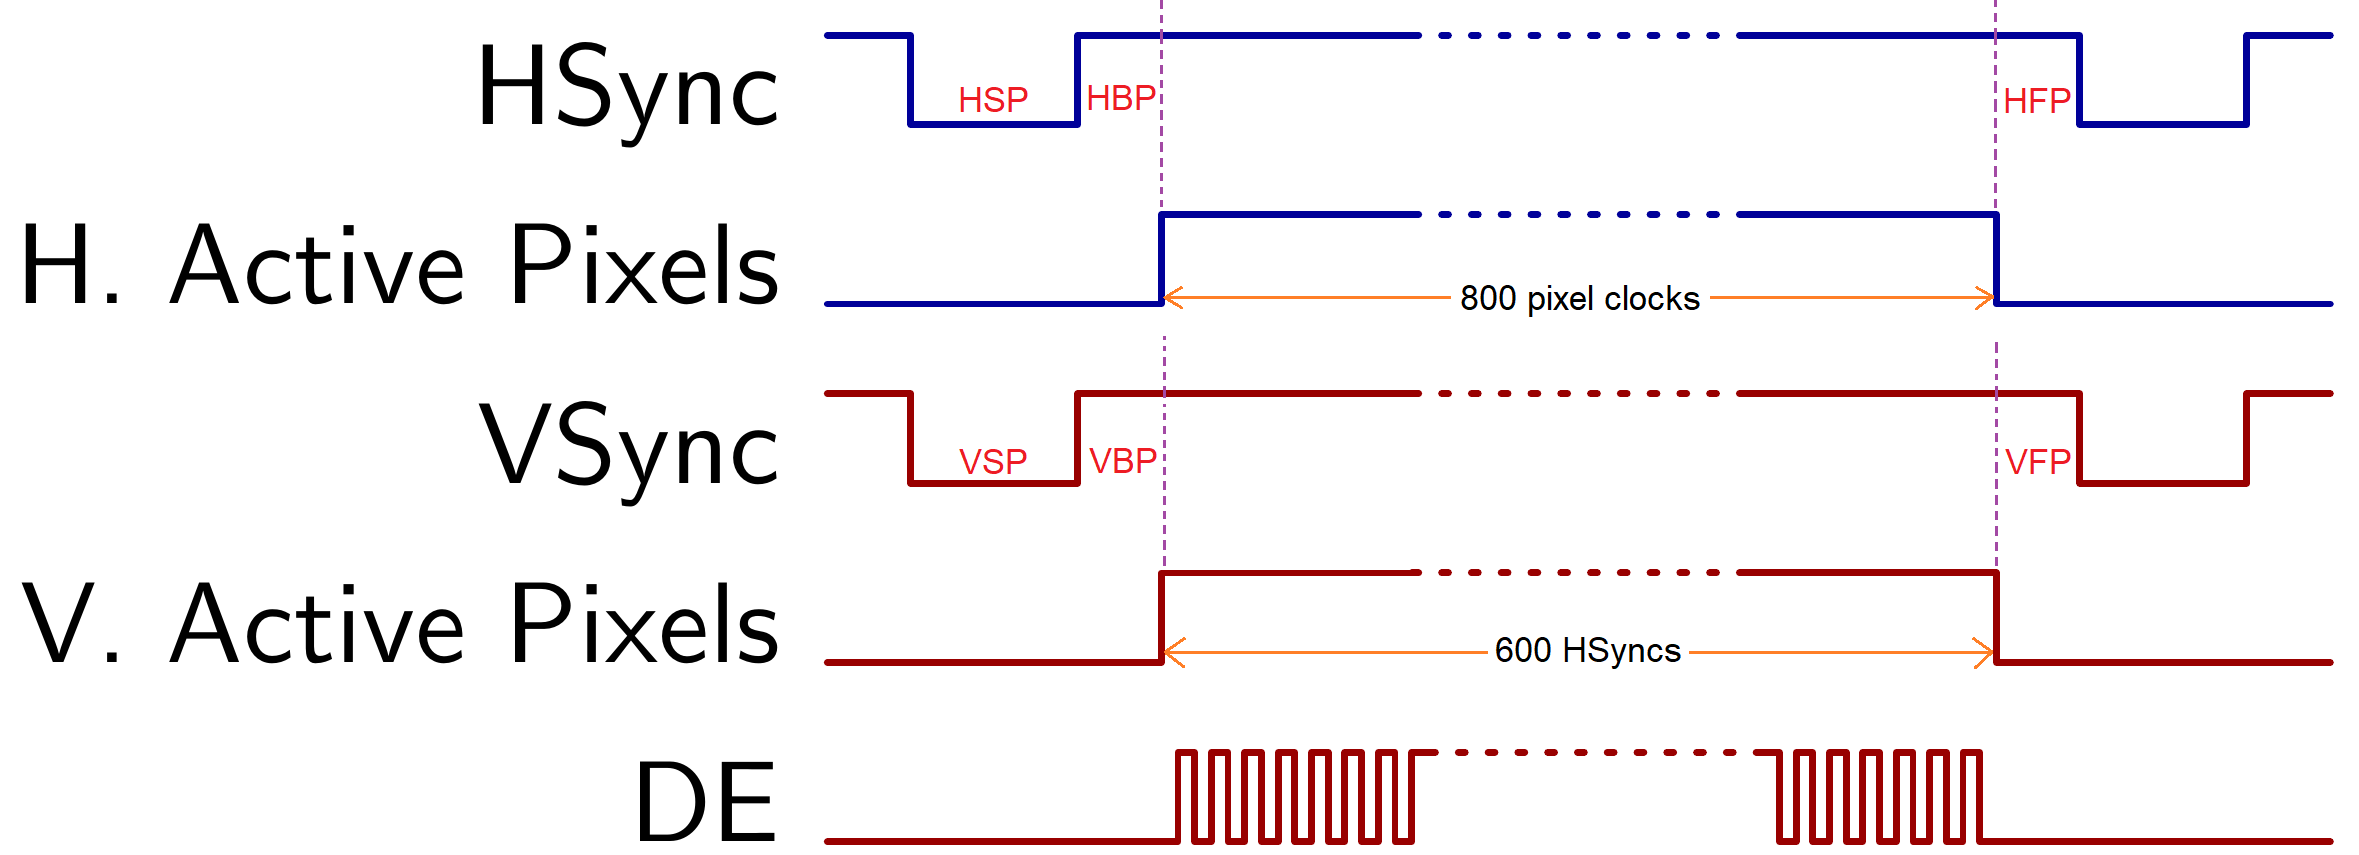
\includegraphics[width=\linewidth]{wf3.png} 
%   \end{tabular}
%   \end{center}
%   \caption{HDMI timing}%[HDMI timing] >>>> use \label inside caption to get Fig. number with \ref{}
%   \label{Fig:1}% Figure captions are used to describe the figure and help the reader understand it's significance.  The caption should be centered underneath the figure and set in 9-point font.  It is preferable for figures and tables to be placed at the top or bottom of the page. LaTeX tends to adhere to this standard.}
%   \end{figure} 

\section{System implementation based on FPGA}
The system diagram is shown in Figure %\ref{}
The system generates structured light patterns at the resolution of $800x600$, the refresh rate of $120 Hz$. According to the document provided by VESA \cite{vesa07}, the HDMI timing should be set as table \ref{Tab:1}.

\begin{table}[!htb]
\caption{HDMI timing of $800x600 @ 120 Hz$}
\label{Tab:1}
\parbox{.45\linewidth}{
\centering
\begin{tabular}{|l|l|}
\hline
\textbf{Pixel Clock} & 73.250MHz \\ \hline
\textbf{Hor. Front Porch} & 48 pixels \\ \hline
\textbf{Hor. Sync Time} & 32 pixels \\ \hline
\textbf{Hor. Back Porch} & 80 pixels \\ \hline
\end{tabular}
}
\hfill
\parbox{.45\linewidth}{
\centering
\begin{tabular}{|l|l|}
\hline
\textbf{Ver. Front Porch} & 3 lines \\ \hline
\textbf{Ver. Sync Time} & 4 lines \\ \hline
\textbf{Ver. Back Porch} & 29 lines \\ \hline
\end{tabular}
}
\end{table}

We utilize an $I^2C$ programmable oscillator Si514 to generate the unusual 73.25MHz pixel clock.
\acknowledgments     %>>>> equivalent to \section*{ACKNOWLEDGMENTS}       
 
This unnumbered section is used to identify those who have aided the authors in understanding or accomplishing the work presented and to acknowledge sources of funding.  

%%%%%%%%%%%%%%%%%%%%%%%%%%%%%%%%%%%%%%%%%%%%%%%%%%%%%%%%%%%%%
%%%%% References %%%%%

\bibliography{report}   %>>>> bibliography data in report.bib
\bibliographystyle{spiebib}   %>>>> makes bibtex use spiebib.bst

\end{document} 
